%% -*- Mode: LATEX -*-

\documentclass[12pt]{../rhitcsse}
\usepackage{multicol}
\usepackage{graphicx}

\ifx\CSSETHREEFIFTYTWO\undefined
\newcommand*{\CSSETHREEFIFTYTWO}{}
\course{CSSE 352}
\coursename{Video Game Development}
\term{Spring}
\acyear{2024-2025}
\instructor{Robert Williamson}
\fi

% Local Variables:
% mode:latex
% End:

 
\title{Lesson 11 Worksheet}

\makeatletter
\renewcommand{\labelenumi}{\bf Question \@arabic\c@enumi}
\makeatother

\begin{document}

\maketitle

\vspace*{0.15in}\hspace{0.25in}Name:\hrulefill\hspace{0.25in}\hspace{0.25in}

\begin{enumerate}
  \item Explain the EventBus pattern (see back) in 2 sentences.
  \vfill
  \item How can we use the EventBus to set up scripts in the right order?
  \vfill
  \item How can you pass arguments to a function call to be used during an EventBus call back?
  \vfill
  \item When might we want more than one EventBus?
  \vfill
  \clearpage
  \centering
  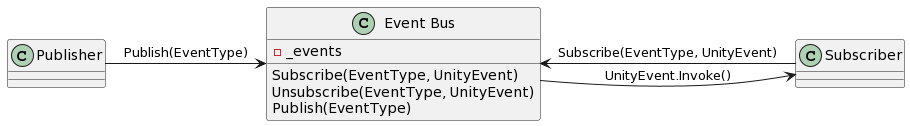
\includegraphics[width=\textwidth]{../figs/EventBus.png}

\end{enumerate}

\end{document}

% Local Variables:
% mode:latex
% End:
